\chapter{Discussie van de resultaten}
\label{discH}
In dit laatste hoofdstuk zullen we een analyse maken van het praktische deel van ons project.
We beginnen met een discussie van de gebruikte methoden en bruikbaarheid van de gevonden resultaten.
Verder worden de resultaten besproken voor het comprimeren van afbeeldingen, het toepassen van het 
Tensorproduct en als laatste het gebruik van de Tensor/Mallat mengvorm op filmmateriaal. 

\section{Discussie}
\subsection{Gebruik van PSNR als maatstaf voor kwaliteit}
Omdat we te maken hebben met lossy beeldcompressie dienen we dit verlies in kaart te brengen op een 
objectieve en kwantitatieve manier. 
De PSNR is een gebruikelijke grootheid voor dit soort analyses: er wordt gezegd dat dit voor eenzelfde 
beginsignaal een goede reflectie geeft van de menselijke beleving van de kwaliteit van de reconstructie.
Uit onderzoek \cite{PSNR} blijkt dat de PSNR een goede maatstaf is zolang er in zeker zin \emph{ceteris paribus}
is aangehouden; voor hetzelfde beeldmateriaal presteert deze maat goed.

\iffalse
\subsection{Bruikbaarheid van resultaten}

De resultaten beslaan slechts een kleine set beelmateriaal: dit heeft vooral met tijdgebrek te maken gehad.
We zullen geen uitspraak doen over de specifieke beeldcategorie\"en uit hoofdstuk \ref{testjes}.
omdat hier simpelweg te weinig studie naar is verricht maar we menen dat de set beelden gevarieerd 
genoeg is om algemene uitspraken te doen over de prestatie van de verschillende algoritmes.
\fi

\subsection{Adaptieve basis}
\label{adaptief_parseval}
We hebben in onze implementatie een adaptieve basis gebruikt: de compressie-algoritme behoudt co\"effici\"enten
die in absolute waarde het grootst zijn. 
We beweren dat dit de beste reconstructie geeft, preciezer: de totale kwadratische fout is zo het kleinst.
We beroepen ons daarvoor op de Parsevalgelijkheid. Wanneer we een selectie $S$ doen van basisfuncties wordt de totale fout na reconstructie
\[
\|f-f|_{S}\|^2_{L_2} = \sum_{k\not\in S} |\inpr{f}{k}|^2 = \sum_{k\not\in S} |c_k|^2,
\]
waar $c_k$ de co\"efficienten is van de basisfunctie $k$. 
Deze sommatie is nu het kleinst wanneer alle termen in de sommatie zo klein mogelijk zijn. 

\section{Compressie van afbeeldingen}

\subsection{Prestatie van Fourier vs. Wavelets}
Uit de PSNR-grafieken blijkt dat de Fouriertransformatie een slechtere reconstructie levert voor 
dezelfde dataset dan zowel de Haar- als de Daubechies-2-wavelettransformaties, 
ongeacht de categorie waartoe het beeld behoort.

\subsection{Wavelet vs. Wavelet}
Tussen de twee wavelets zien we verder wat we theoretisch verwachten: Haar presteert goed bij harde randen
vanwege zijn kleine drager terwijl Daubechies voor vloeiend/fotografisch materiaal een goede reconstructie geeft.

\subsection{Convergentie bij kleine dataset}
Uit de grafiek blijkt dat het verschil in kwaliteit tussen de verschillende compressie algoritmes afneemt wanneer
de hoeveelheid data die opgeslagen wordt, kleiner wordt. 
Door de kleine dataset is de willekeur van de vorm van het plaatje erg van invloed op kwaliteit van de reconstructie 
voor verschillende algoritmes. 
Ook is het dubieus of de PSNR nog een goede maatstaf is voor de menselijke perceptie wanneer de algoritmes
zo'n slechte maar zeer verschillende benadering geven van het originele beeld.
We zullen daarom hier geen uitspraak over kunnen doen.

\section{Het Tensorproduct op afbeeldingen}
Voor de volledigheid hebben we er voor gekozen \'o\'ok het Tensorproduct te bekijken bij een aantal 
van onze afbeeldingen: zie figuren \ref{fig:tensor_start}-\ref{fig:tensor_end}. We hebben er voor 
gekozen om niet alle afbeeldingen in dit formaat weer te geven: deze twee afbeeldingen geven een goede representatie.

Het eerste wat op te merken valt, zijn de horizontale en verticale balken die bij het Tensorproduct 
tevoorschijn komen. Deze zijn in de Mallatdecompositie een stuk minder aanwezig. De reden 
hiervoor is simpel aan te wijzen. Bij de Mallatdecompositie bekijken we wavelets met een 
drager die in beide richtingen even groot is (een vierkant dus). Het Tensorproduct legt deze eis 
niet op met als gevolg dat er een wavelet is met een drager die heel breed is en ook weer 
heel kort: een balk. Als deze balk door de compressie-algoritme weggelaten wordt, mist de 
reconstructie hier een benadering en kan er een gekke horizontale/verticale balk in de reconstructie onstaan.

Het tweede wat we opmerkten is dat de PSNR structureel lager is bij het Tensorproduct in vergelijking 
met de Mallatdecompositie. Dit komt ook wel overeen met wat we zien in de figuren \ref{fig:tensor_start} 
en \ref{fig:tensor_end}. Merk wel op dat vooral figuur \ref{fig:tensor_start} een extreem voorbeeld 
is en dat de verschillen in figuur \ref{fig:tensor_end} al een stuk minder overheersend zijn.

Het is interessant om op te merken dat onze metingen -- dat het Tensorproduct consistent lagere 
PSNR-waardes oplevert -- in strijd zijn met de claims die gemaakt worden in \cite{tensor_vs_mallat}, 
hoewel er teveel onbekende factoren zijn om te weten of dit misschien een andere reden heeft.

\section{Gemengde decompositie op 3D signalen}
Het bekijken van 3D signalen was een interessante toevoeging aan ons project maar de analyse  
van filmmateriaal is moeilijker gebleken. Dit had twee redenen.

Ten eerste is onze implementatie, hoewel effici\"ent, niet erg snel. Het comprimeren van een 
afbeelding duurt ongeveer dertig seconden en het comprimeren van filmmateriaal duurt al snel het 
vijftigvoudige. Hierdoor wordt het comprimeren van voldoende 3D signalen een langdurige taak.

Daarnaast hebben we veel moeite gehad om passend beeldmateriaal te vinden. Uit het eerste punt volgt 
dat dit beeldmateriaal klein in afmeting moet zijn. Als de afbeelding klein is, is het echter moeilijk
om een bepaalde compressie-ratio te halen met een goede reconstructie. Dit maakte de zoektocht lastig.

\subsection{PSNR}
Hoewel de PSNR in het geval van de afbeeldingen een prima representatie geeft van de kwaliteit van de 
reconstructie, blijkt het bij het beeldmateriaal dat wij bekeken hebben minder goed te werken. 
Zie bijvoorbeeld de grafiek links in \ref{fig:cockto}, hier is te zien dat de PSNR slechts weinig verschilt
tussen de verschillende compressieniveau's zodat we geen nuttige conclusies kunnen trekken.
Daarentegen zien we in grafiek rechts in \ref{fig:cockto} een patroon dat we verwachten, daling van de PSNR
bij kleinere compressiepercentages.

Aangezien we niet erg veel beeldmateriaal bekeken hebben zullen we de PSNR als maat loslaten en ons richten 
op de optische verschillen die we kunnen aanwijzen tussen de twee reconstructies.

\begin{figure}[h]
\centering
\begin{subfigure}[t]{0.48\textwidth}
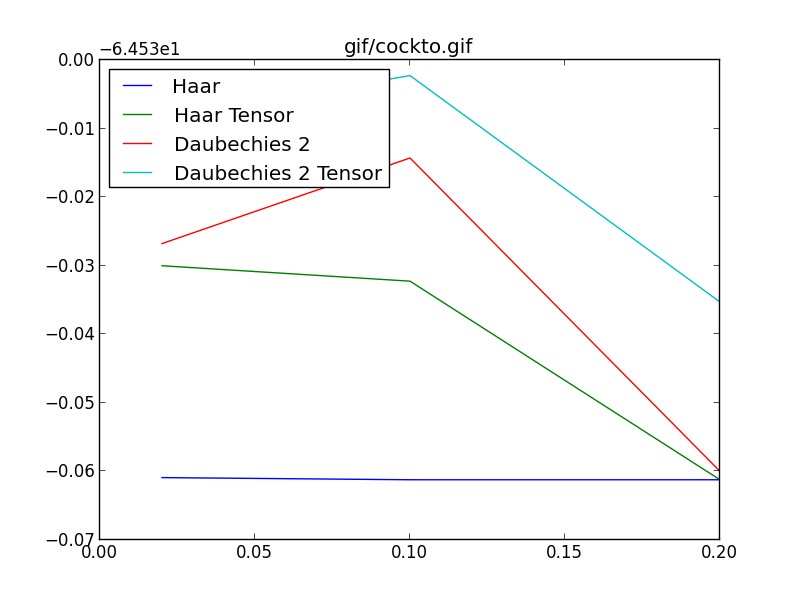
\includegraphics[width=\linewidth]{plaatjes/cockto.png}
\end{subfigure}
\begin{subfigure}[t]{0.48\textwidth}
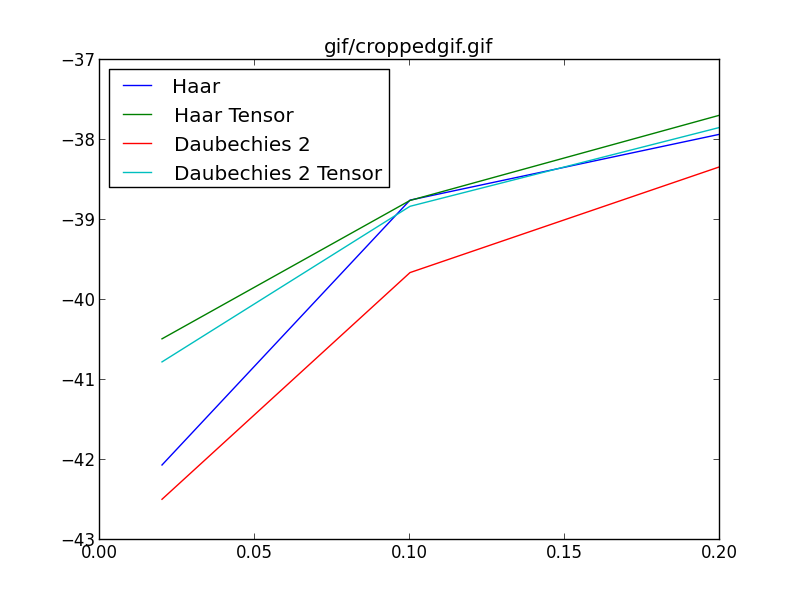
\includegraphics[width=\linewidth]{plaatjes/croppedgif.png}
\end{subfigure}
\caption{Links: de grafiek horende bij de dansende octopus. Rechts: de grafiek horende bij de scene met de typmachine en de boom.}
\label{fig:cockto}
\end{figure}

\subsection{Mallatdecompositie versus de mengvorm}
Wat we wel direct opmerkten is het enorme verschil in detail tussen de twee compressiemethoden. 
Dit komt omdat het Tensorproduct sneller convergeert bij continue signalen 
(zie stellingen \ref{thm:foutmallat} en \ref{thm:fouttensor}). 
Omdat een bewegend beeld over het algemeen continu is in de tijdsdimensie, is het gevolg niet vreemd.

Wanneer er w\'el een grote sprong in de tijd optreedt, zoals bij een scenewisseling, is de fout van 
het Tensorproduct ineens een stuk groter dan die van de Mallatdecompositie. 
Dit is vooral duidelijk bij de typmachinescene, die voor de Mallatdecompositie en de mengvorm
weergegeven is in figuren \ref{fig:frames_tensor} en \ref{fig:frames_nontensor}.
Het gele mannetje vervaagt in de Mallatdecompositie gedurende ongeveer 5 tijdseenheden 
terwijl de randen in de mengvorm voor 7 frames zichtbaar blijven.

Dit resultaat is ten eerste te wijten aan de grote(re) drager van de Daubechieswavelet, 
waardoor harde randen slechter gereconstrueerd worden.
Het effect wordt echter versterkt in de mengvorm doordat hier veel wavelets een langwerpige
drager in de tijdsrichting hebben, wanneer de scherpe randen in frame $71$ gereconstrueerd moeten worden
zijn deze ook goed te zien in de volgende frames.

\begin{figure}[h]
\centering
\begin{subfigure}{\linewidth}
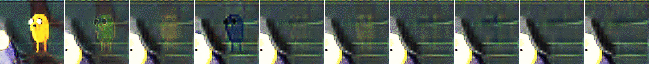
\includegraphics[width=\linewidth]{plaatjes/frames_notensor_small.png}
\caption{Mallatdecompositie}
\label{fig:frames_tensor}
\end{subfigure}
\centering
\begin{subfigure}{\linewidth}

\includegraphics[width=\linewidth]{plaatjes/frames_tensor_small.png}
\caption{Mengvorm}
\label{fig:frames_nontensor}
\end{subfigure}
\caption{\texttt{croppedgif.gif} (met verhoogd contrast) ingezoomd op de verstoring, frames 71 t/m 80 met 2\% compressie door de Daubechies 2-wavelet
met de verschillende decomposities.}
\end{figure}
